% !TEX root = ../paper.tex
\doclearpage
\section{Overview of \texorpdfstring{$\truthtable$}{TruthTable}}
\label{sec:overview}

Our protocols extend $\truthtable$~\cite{cryptoeprint:2026/1260}; therefore, we recall in this section the system model that $\truthtable$ realizes and the structure of its construction, and point out where each of our contributions enters. The material in this section is due to $\truthtable$; we refer the reader to its paper for the full treatment.

\parhead{System model for verifiable databases}
A verifiable database system involves three parties: a \emph{trusted} database owner $\DataOwner$ who holds a database $\Database$, an \emph{untrusted} database server $\Server$, and a client $\Client$.
These parties interact as follows.
\begin{enumerate}[nosep]
    \item The database owner $\DataOwner$ generates a cryptographic commitment $\DatabaseCM$ to the database $\Database$, and sends $\DatabaseCM$ to both $\Client$ and $\Server$ (or equivalently, posts it to a public ledger).
    $\DataOwner$ also sends the database $\Database$ to $\Server$.
    At this point, $\DataOwner$'s job is done, and it can go offline.
    \item $\Client$ issues a query $\Query$ to $\Server$. The latter executes $\Query$ on $\Database$, and additionally generates a cryptographic proof $\Proof_\Query$ certifying that the query result is correct with respect to the committed database $\DatabaseCM$.
    \item $\Server$ sends both $\QueryResult$ and $\Proof_\Query$ to $\Client$, who verifies the proof $\Proof_\Query$ to confirm that $\QueryResult$ is indeed the correct query result.
\end{enumerate}
The preprocessing of \cref{sec:preprocessing} lives entirely in the first step: the fingerprint and rank columns are computed and committed by $\DataOwner$ together with the data, before it goes offline.

\parhead{Definition of verifiable databases}
Formally, a verifiable database system is a commit-carrying SNARK (cc-SNARK)~\cite{CampanelliFQ19} for the following ternary relation:
{\small
\begin{displaymath}
 \Relation{\SQL} = \left\{\,
    (
        \NPInstance = (\Query, \QueryResult),
        \NPInstancey = \Database,
        \NPWitness = \bot
    )
  \;\middle|\;
  \QueryResult \in \ResultSet_\Query(\Database)
\,\right\},
\end{displaymath}
}

\noindent
where $\ResultSet_\Query(\Database)$ denotes the set of valid query results for the query $\Query$ on the database $\Database$ with respect to SQL semantics.
In a ternary relation, $\NPInstance$ denotes the explicit instance, $\NPInstancey$ the implicit instance, and $\NPWitness$ the witness; the distinction between explicit and implicit instances separates the parts of the instance that the cc-SNARK verifier reads entirely ($\NPInstance$) from those it reads only in committed form ($\NPInstancey$).
The cc-SNARK algorithms specialized to this relation are:
\begin{itemize}[nosep]
    \item $\Setup(1^\lambda, N) \rightarrow (\pk, \vk, \ck)$, on input a database size $N$ and security parameter $\lambda$, outputs a prover key $\pk$, verifier key $\vk$, and commitment key $\ck$.
    \item $\Commit(\ck, \Database) \rightarrow \DatabaseCM$, on input a database $\Database$, outputs a commitment $\DatabaseCM$ to the database.
    \item $\Prove(\pk, \Database, \DatabaseCM, \Query, \QueryResult) \rightarrow \Proof_\Query$, on input a database $\Database$, the database commitment $\DatabaseCM$, a query $\Query$, and the query result $\QueryResult$, outputs a proof $\Proof_\Query$ that $\QueryResult$ is the result of executing $\Query$ on $\Database$.
    \item $\Verify(\vk, \DatabaseCM, \Query, \QueryResult, \Proof_\Query) \rightarrow \{0,1\}$, on input a database commitment $\DatabaseCM$, a query $\Query$, a query result $\QueryResult$, and a proof $\Proof_\Query$, accepts if the proof is valid.
\end{itemize}
These algorithms must satisfy the standard completeness and knowledge-soundness properties of cc-SNARKs~\cite{CampanelliFQ19}; see \cref{sec:extended_preliminaries}.

\subsection{Construction Strategy}
\label{sec:overview:construction-strategy}

We now describe how $\truthtable$ realizes the commitment, prover, and verifier algorithms.

\parhead{Commit}
$\truthtable$ represents SQL tables as tuples of (multilinear) polynomials, and commits to these via a polynomial commitment scheme~\cite{KateZG10}.
Each column is represented as a separate polynomial, so the size of a table commitment, and the cost of producing it, is the number of columns times that of a single column.
The polynomial encoding of a table $\Table$ is called its \emph{arithmetization}, denoted $\hat{\Table}$; the same hat convention extends to columns and other table-derived objects throughout the paper.
The encoding is designed so that efficient protocols can check that SQL operators were correctly applied to the encoded tables.
\Cref{sec:arithmetization} recalls this encoding and presents our extension of it to string columns, which adds the auxiliary polynomials that the rest of the paper operates on; the extra commitments are produced at this step.

\parhead{Prover and verifier}
To check that a claimed instance $(\Query, \QueryResult)$ is valid for a committed database $\Database$, i.e.\ $((\Query, \QueryResult), \Database) \in \Relation{\SQL}$, $\truthtable$'s prover and verifier proceed in three steps.
First, they invoke a parser to transform the query $\Query$ into a \emph{query plan} $\QueryPlan$, a tree representation of the query that makes analysis and optimization easier.
Next, both invoke the query planner to optimize the plan.
Finally, both invoke the proof engine on the optimized plan: they traverse it node by node and execute subprotocols that prove the correctness of each node.

A \textbf{query plan} $\QueryPlan$ for a query $\Query$ is a tree whose nodes represent relational operators (e.g.\ filter, join, limit) and whose edges represent the flow of data between them; edges into the leaves carry the input database tables, and the edge leaving the root carries the output table.
\Cref{fig:example-qp} depicts the query plan obtained by parsing the query in \cref{fig:example-query}.
The modular nature of plans makes protocol construction and analysis simpler: instead of $\Relation{\SQL}$, $\truthtable$ works with the equivalent relation
{\small
\begin{displaymath}
 \Relation{\QueryPlan} = \left\{\,
    (
        \NPInstance = (\QueryPlan, \QueryResult),
        \NPInstancey = \Database,
        \NPWitness = \bot
    )
  \;\middle|\;
  \QueryResult \in \ResultSet_\QueryPlan(\Database)
\,\right\}\enspace,
\end{displaymath}
}

\noindent
which is equivalent to $\Relation{\SQL}$ because a claimed output is the correct result of a query if and only if it is the result of executing the corresponding plan.

\begin{figure}[htbp]
\centering
\begin{subfigure}[b]{0.56\linewidth}
    \centering
    \begin{lrbox}{\sqlbox}%
\begin{lstlisting}[style=sql]
SELECT * FROM users
 JOIN orders
   ON users.id = orders.id
WHERE orders.amount > 100;
\end{lstlisting}
    \end{lrbox}%
    \usebox{\sqlbox}
    \caption{Example SQL query.}
    \label{fig:example-query}
\end{subfigure}\hfill
\begin{subfigure}[b]{0.42\linewidth}
    \centering
    \includegraphics[page=3, scale=0.5]{figures/cropped_figs.pdf}
    \caption{Query plan}
    \label{fig:example-qp}
\end{subfigure}
\caption{Query plan (b) for query (a).}
\label{fig:pfqp}
\end{figure}

\subsection{Proof Engine}
\label{sec:overview-proof-engine}

The query planner first rewrites $\QueryPlan$ into an equivalent plan $\QueryPlan_\opt$ that is cheaper to prove.
On input $\QueryPlan_\opt$, the proof engine constructs a protocol for proving that $((\QueryPlan_\opt, \QueryResult), \Database) \in \Language{\QP}$.
$\truthtable$ designs a Polynomial Interactive Oracle Proof (PIOP)~\cite{ChiesaHMMVW20,BunzFS20} for this relation and compiles it to a succinct argument with the same polynomial commitment scheme used in the commit phase; the compilation is standard, so the paper, like ours, focuses on the PIOPs.

The prover first generates a \emph{table assignment} $\{\Table_i\}_{i=1}^m$ of intermediate result tables labelling the $m$ non-leaf edges of the plan, encodes them as polynomials, and sends their oracles to the verifier.
Then, for each node $\nu$ of the plan, the prover and verifier engage in a sub-PIOP asserting that the output table oracle $\TableOut_\nu$ is a valid result of executing $\nu.\op$ on the input table oracles $\{\TableIn\}_\nu$.\footnote{Since an operation may admit several correct results, the output table is required to lie in the set of possible results $\ResultSet_{\nu.\op}(\{\TableIn\})$.}
Finally, the prover and verifier engage in a \emph{result check} to verify that the root oracle opens to the purported query result $\QueryResult$.
Each node-specific sub-PIOP proves membership in a ``node relation'' that restricts $\Relation{\QP}$ to the operation of that node; for a filter with predicate $p$, for instance, the relation requires that every row of $\TableOut$ appears in $\TableIn$, that every row of $\TableOut$ satisfies $p$, and that every row of $\TableIn$ absent from $\TableOut$ fails $p$.\footnote{Precisely, the sub-PIOPs prove ``arithmetized'' versions of the node relations, in which each table is replaced by its arithmetization; see \cref{sec:arithmetization}.}
The strategy is complete and sound as long as the per-node checks are, which $\truthtable$ proves formally.
Our operator protocols for pattern matching (\cref{sec:piop-for-pattern-matching}) and ordering (\cref{sec:lex-order}) are exactly such node sub-PIOPs, for the filter and sort nodes whose predicates and keys involve string columns, and the consistency checks of \cref{sec:string-toolbox} accompany every node whose output carries a string column.
